\section{Approach}

\begin{figure}[t]
  \centering
  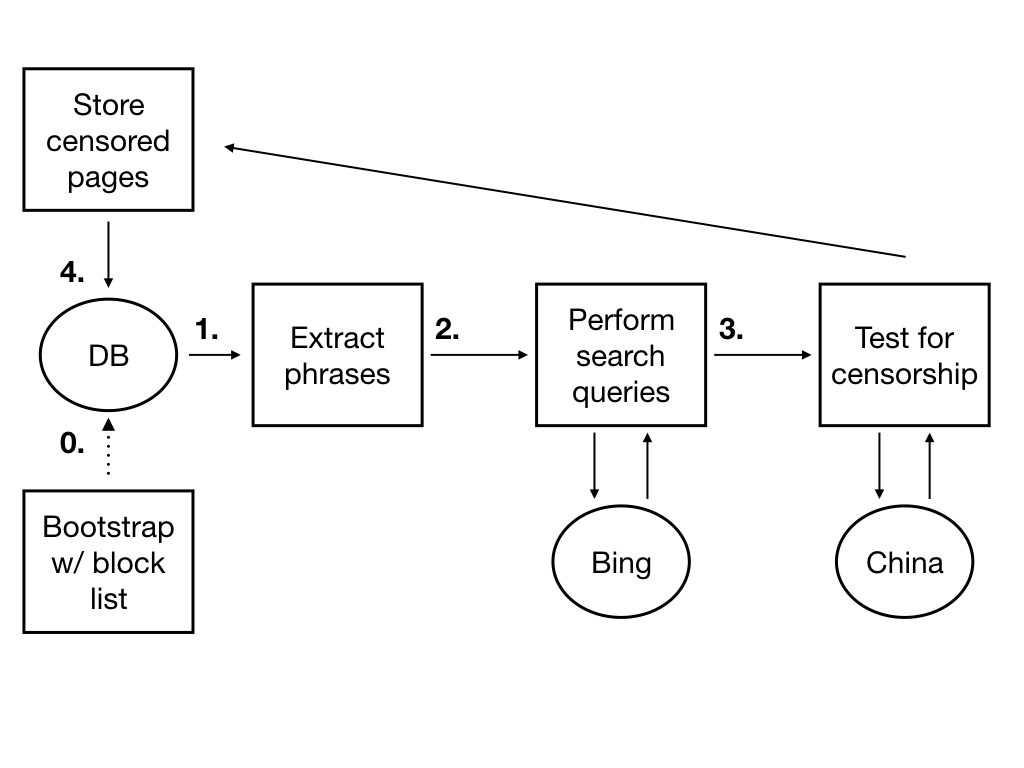
\includegraphics[scale=0.23]{figures/arch-2}
  \caption{\label{arch}Our approach for discovering censored websites.}
\end{figure}

Figure~\ref{arch} summarizes our approach to finding censored
websites. For the most part, our approach is similar to that of
FilteredWeb~\cite{darer2017filteredweb}. We start by bootstrapping a
list of web pages that are known to be censored, such as the Citizen
Lab block list~\cite{citizenlab:block}.  Then, we extract Chinese and
English phrases that characterize these web pages.  Then, we use these
phrases as search queries to find related web pages that might also be
censored. Finally, we test each search result for DNS manipulation in
China and feed the censored web pages back to the beginning of the
system. The rest of this section details the new capabilities of our
approach beyond the state of the art.

\subsection{Extracting multi-word phrases}
An n-gram is a building block for natural-language processing that
represents a sequence of ``n'' units of text, e.g. words. For example,
if we were to compute all of the bigrams of words in the English
phrase \texttt{Chinese human rights violation}, we'd get
\texttt{Chinese human}, \texttt{human rights}, and \texttt{rights
violation}. Similarly, if we were to compute all the trigrams of
words, we'd get \texttt{Chinese human rights} and \texttt{human rights
violation}. On the other hand, if we simply extract unigrams from the
sentence, we'd be left with \texttt{Chinese}, \texttt{human},
\texttt{rights}, and \texttt{violation}. As such, we believe that by
extracting content-rich unigrams, bigrams, trigrams, we're able to
learn more about the subject of a web page.

Unfortunately, computing the n-grams of words in Chinese text is
difficult because it is typically written without spaces, and there is
no clear indication of where characters should be separated. Computing
such boundaries in natural-language processing tasks is often
probabilistic, and depending on where characters are separated, one
can arrive at very different meanings for a given
phrase~\cite{stanford:segmenter}. For example, consider the
text \begin{CJK*}{UTF8}{gbsn}天花\end{CJK*}. This is considered a
Chinese unigram that translates to
``smallpox'' in English, but the character \begin{CJK*}{UTF8}{gbsn}
天\end{CJK*} on its own translates to ``sky'', and the
character \begin{CJK*}{UTF8}{gbsn}花\end{CJK*} on its own translates
to ``flower''. Given that we do not have domain-specific knowledge of
the web pages that we're analyzing, we consider a unigram to be
whatever the segmenter software in the Stanford CoreNLP library considers to be
a unigram.~\cite{tseng2005conditional, chang2008optimizing}.

We believe that using Chinese unigrams, bigrams, and trigrams for search queries
instead of individual English words is more effective for discovering
censored websites in China. For example, we know that websites that
express collective dissent are considered sensitive by the Chinese
government~\cite{king2013censorship}. If we used the words
\texttt{destroy}, \texttt{the}, \texttt{Communist}, or \texttt{Party}
individually as search terms, we might not get websites that express
collective dissent because the words have been taken out of
context. On the other hand, the phrase ``\texttt{destroy the Communist
Party}'' as a whole expresses collective dissent, which might enable us
to find many censored domains when used as a search term. We evaluate
the effectiveness of such phrases in Section \ref{phrases-eval}.

\subsection{Ranking phrases} \label{tf-idf}
To ``rank'' the phrases on a censored web page, we use
term-frequency/inverse document-frequency (TF-IDF). TF-IDF is a
natural language technique that allows us to determine which phrases
best characterize a given web page~\cite{ramos2003using}. It can be
thought to work in three steps. First, we compute the term-frequency
for each phrase on a web page, which means that we count the frequency
of each unigram, bigram and trigram. Then, we compute the document-frequency
for each phrase on a web page, which entails searching a Chinese corpus
for the frequency of a given phrase across all documents in the
corpus~\cite{phrasefinder}. Finally, we multiply the term frequency by
the inverse of the document frequency. The resulting score gives us an
idea of how important a given Chinese phrase is to a web page.

Using this method, phrases like \begin{CJK*}{UTF8}{gbsn}1989年民主运
动\end{CJK*} [\texttt{1989 democracy movement}]
and \begin{CJK*}{UTF8}{gbsn}天安门广场示威\end{CJK*}
[\texttt{Tienanmen Square Demonstrations}] might rank highly on a
website about Chinese political protests. We would then use these phrases
as search terms in order to find related websites that might also be
censored. If we find a lot of censored URLs as a result, then we can
infer that the topic covered by that phrase is considered sensitive in China.

\subsection{Parsing Chinese text}
Before we can compute TF-IDF for a given web page, we need to tokenize the
text. Doing so is simple enough for English because each word is separated by a
space. For languages such as Chinese, however, all of the words in a sentence are
concatenated, without any spaces between them. As such, we need to apply
natural-language processing techniques to perform fine-grained analysis
of the text on a web page.

To do so, we make use of Stanford CoreNLP, a set of natural language
processing tools that operate on text for English, Arabic, Chinese, French,
German, and Spanish~\cite{corenlp2016suite}. For Chinese web pages, it allows us
split a sentence into a sequence of unigrams, each of which may represent
one word or even multiple words. By combining neighboring unigrams, then, we
can extract key phrases from a web page that describe its content.

As previously mentioned, although FilteredWeb is concerned with finding web pages
that are censored in China, it is only able to parse text for the ISO basic
Latin alphabet~\cite{darer2017filteredweb}. By being able to parse Chinese text as
well as ISO Latin text, then, we are able to cover many more web pages and
extract regional information that may explain why a given web page is
censored. In future work, we could make use of more intricate tools
from Stanford CoreNLP likes its part-of-speech tagger to identify
phrases that convey relevant information.
